\chapter{Identification of enriched regions using peak calling}

\section{Building a signal profile.}

\begin{figure}[b!]
    \centering
    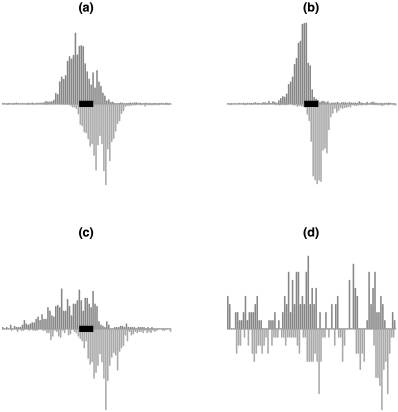
\includegraphics[width=\textwidth]{../img/peaks.jpg}
    \captionsource{Illustration of individual reads mapping to the forward (up) and reverse (down) strand, building the good binding site prfile (a, b, c) and false positive (d). }{doi: 10.1371/journal.pone.0089694}
    \label{fig:graph_classes}
\end{figure}

The computational method of the protein-chromatin binding event identification plays a central role in ChIP-seq analysis. 
After read mapping to the reference, the next step is to identify loci with high read density comparatively to the background, referred to ChIP-seq signals, or simply peaks.
More than 30 algorithms and tools have been implemented to solve that computational problem~\cite{chen2012systematic}.
The choice of the right peak caller is crucial and depends on the type of experiment~\cite{nakato2017recent}, e.g. TF binding event identification vs. long-range histone marks interactions.



Suitable software builds a peak profile along each chromosome. 
All the peak profiles can be divided into three categories~\cite{park2009chip}. 
Sharp peaks are typical for TF due to dependency on motif sequence~\cite{landt2012chip}. 
Histones have non-specific positioning on the DNA~\cite{krig2007identification}. 
Thus the peak profile is broad and can reach several kilobases. 
The third peak type is a mix of sharp and broad signals, a typical pattern for RNA polymerase II and transcription elongation factor~\cite{squazzo2006suz12, lin2011dynamic}.
% \todo{to je zavádějící. Nukleosomy sice nevážou konkrétní motiv DNA, ale vykazují jistou míru sekvenčních preferencí, která se liší v závislosti na organismu.}



The very first extended set methodology to calculate peak profile density was presented in 2007~\cite{robertson2007genome}. 
Fragments are sequenced from 5' to 3' end, and the minimal enough length of a sequenced read is 36 bp long. 
But the real fragment of DNA is longer, and thus the interaction of the protein of interest is somewhere on that size selected long DNA fragment. 
Each read is computationally extended in the 3' direction. 
Regions are scored by the number of overlap reads and assessed as a candidate peak.



Sequence directionality sets the stage for a smoothed profile. 
The strand-specific read distribution form bimodal pattern combined by shifting or extending tags toward the center~\cite{valouev2008genome}.
\todo{obrázek by možná čtenářům pomohl snáze pochopit popisované kroky}

%%%%%%%%%%%%%%%%%%%%%%%%%%%%%%%%%%%%%%%%%%%%%%%%%%%
\section{Statistical model utilization for the assesment of the significance of estimated signals.}


Standard biological research has some rate of false positives. 
Due to there is no absolute proof or absolute rejection of the results in ChIP-seq studies, the analysis works with probabilities.
The end goal of the ChIP-seq experiment is the genomic loci of possible protein binding events. 
The end goal of the ChIP-seq experiment is to define the genomic loci of possible protein binding events. 
The candidate signal of a binding event is represented as a hypothesis $H_{1}$, and the null hypothesis $H_{0}$ is that there is no actual binding. To describe the statistical significance of the individual hypothesis, a P-value is calculated. 

The early approach was that the background noise is uniform; 
however, the usage of the control dataset shows that the different biases make uniform model is too ideal to be true~\cite{robertson2007genome}. 
That is why all peak calling algorithms make all the output signals associated with P-value~\cite{chitpin2019recap} to determine statistical significance in a hypothesis test. 
The null hypothesis's incorrect rejection produces the Type I error known as a "false positive". 
In the contest of ChIP-seq analysis, this type of error occurs when there is no actual binding event, but the peak caller shows that there is. 
The inversion of Type I error is Type II error, which is referred to as a "false negative". 
Considering the ChIP-seq experiment, the "false negative" error type is seen less serious than "false positives". 
\todo{proč to tak je? a můžeš své tvrzení podpořit nějakou citací?}

To test peaks for significance, different peak calling algorithms adopt different statistical techniques. 
In a MUSIC's approach~\cite{harmanci2014music}, a window of fixed size for TF or varying width for histone marks while scanning a genome ranks the candidate peaks using a Binomial test, where the distribution of the total number of mapped tags in the respective regions across IP and control is assumed to be equal:

\begin{align*}
    p_{k,n} = \binom{n}{k}p^k(1-p)^{n-k}
\end{align*}

The widely used Poisson model was utilized in early software tools such as SICER~\cite{zang2009clustering}. 
The Poisson is directly connected to Binomial distribution,
where probability \textit{p} of succes in each trail and p$_{k,n}$  for \textit{k} succes in \textit{n} trails; but assosiated with rare events:

\begin{align*}
    p_{0,n} = (1 - p)^{n} = \left(1-{\frac{\lambda}{n}}\right)^{n} \to e^{-\lambda}
\end{align*}

\begin{align*}
    p_{1,n} = np(1 - p)^{n-1} = \frac{\lambda}{1-p}\left(1-{\frac{\lambda}{n}}\right)^{n} \to \lambda e^{-\lambda}
\end{align*}

\begin{align*}
    p_{2,n} = \frac{1}{2} n(n - 1) p^{2} (1-p)^{n-2} = \frac{1}{2} \frac{\lambda^{2} - \lambda p}{ (1-p)^{2}} \left(1-{\frac{\lambda}{n}}\right)^{n} \to \frac{1}{2} \lambda^{2} e^{-\lambda}
\end{align*}

For \textit{k} succes in \textit{n} trails with probability p=${\lambda / n}$ , the binomial probability p$_{n,k}$ approaches the Poisson probability:

\begin{align*}
    P_k = \frac{\lambda _i ^{k}}{k!} e^{- \lambda _i}
\end{align*}

The Poisson parameter $\lambda_i$ is supposed to be constant across the genome and provided to be inadequate for ChIP-seq peak calling to identify TFs binding sites. 
The negative binomial model was suggested by CisGenome~\cite{ji2008inte}, which is, in fact, a generalization of the Poisson distribution, also known as the gamma-Poisson mixture distribution. 

\begin{align*}
    NB_{y_i; \mu _i, \alpha} = \frac{\Gamma (y_i + \alpha ^{-1})}{\Gamma(\alpha ^{-1})\Gamma(y_i + 1)} \left(\frac{\alpha ^{-1}}{\alpha ^{-1} + \mu_i}\right) ^{\alpha ^{-1}} \left(\frac{ \mu _i}{ \alpha ^{-1} + \mu _i}\right) ^{y _i}
\end{align*}

The derevation from two-parameter gamma distribution is done in on page 118 in~\cite[Cameron and Trivedi (2013)]{cameron2013regression}.

Another suggestion was to estimate $\lambda$ for each genomic position by the local Poisson test. 
Such an approach was introduced by the most popular peak caller called MACS~\cite{zhang2008model}.
The tool slides with a constant size window centered on each nucleotide across the genome, merge overlapping peaks by extending the read.
If the number of reads in the IP sample is higher than expected, given a background rate estimated from the control dataset, then using the Poison test, the enriched regions are ranked~\cite{thomas2017features}. 
The highest tag pileup is defined as a summit of a signal.  

Comparing the statistical models implemented by different peak calling algorithms shows that the Poisson test is a better approach to score the candidate signals than the Binomial test~\cite{thomas2017features}.

%%%%%%%%%%%%%%%%%%%%%%%%%%%%%%%%%%%%%%%%%%%%%%%%%%
\section{Multiple hypothesis testing and reliability of the result.}

After scanning through the genome and find a large number of candidate regions estimating null distribution, the quality of the detected peaks should be identified. 
From generated data, the candidate signal may be either a false or true binding event. 
And the probabilistic statement cannot be made by using a well known Bayes' Theorem. 
In the genomic studies, especially in ChIP-seq, individual hypothesis testing is not useful, and a global hypothesis test is required~\cite{futschik2019omnibus}. 

Suppose we have \textit{n} genomic loci obtained.
The $i^{th}$ null hypothesis $H_{0,i}$ with corresponding P-values $p_i$.
The global null hypothesis of simultenious test of all null hypitheses  is defined:

\begin{align*}
    H_0 = \displaystyle\bigcap_{i=1}^{n} H_{0, i}
\end{align*}

Fisher's combined probability test~\cite{fisher1992statistical} combines known P-values:

\begin{align*}
    T = - \displaystyle \sum_{i=1}^{n} 2 \log p_i \sim  \chi_{2n}^{2}
\end{align*}

Bonferroni's test~\cite{hommel1988stagewise} looks at the smallest P-value and at given desired level $\alpha$ tests the global null hypothesis by testing each $H_{0,i}$ at level $\alpha /n$. 
And whenever $p_i \leq \alpha / n$ rejects the global null hypothesis.
Assuming the global hypothesis is true, the overal level control is: 

\begin{align*}
    P_{H_0}[Error Type I] = P_{H_0} \left[\bigcup_{i=1}^{n} \left\{ p_i \leq \alpha / n\right\}\right] \leq \sum_{i=1}^{n} P_{H_0}(p_i \le \alpha / n)  = n \frac{\alpha}{n} = \alpha
\end{align*}

\todo{pro Fishera a FWER chybí citace}
Even though both tests are easy and straightforward, non of them is effective. 
Fisher's test will be eliminated in a large number of the true null hypothesis. 
In the case of  Bonferroni's test, the only one P-value is used. 
Hence it can be applied only if very few binding events are expected to be significant. 
The rejection of extreme value of binding event at the $\alpha$ significance level leads to increase number of false positives. 
The idea of the global null hypothesis rejection is not suitable for genomic analysis. 
Another approach is the familywise error (FWER) rate method:

\begin{align*}
    FWER \leq 1 - (1 - \alpha)^c, 
\end{align*}

where $\alpha$ is a level for an individual test, $c$ is a number of comparisons.
The test controls the probability of performing one or more Type I errors. 
However, the method is very conservative and does only a few rejections. 

The application of the False Discovery Rate (FDR) approach in the genomic field is associated with microarray technology~\cite{lai2017statistical}.
The method allows a few small rejections if the majority of the rejections are correct. 
\todo{nerozumím, co znamená "SMALL rejection"}
Such testing adjusts the statistical confidence based on the number of tests. 

Let $R$ be the total number of rejections and $V$ be the number of trully null hypotheses.
The the proportion $Q$ of false positive rejection among all rejection is 

\begin{align*}
    Q = \frac{V}{R} .
\end{align*}

The Benjamini-Hochberg procedure~\cite{benjamini2000adaptive} ensures the expectetion and define False Dicovery Rate as follow: 

\begin{align*}
    FDR = E(Q) = E \left(\frac{V}{R}\right) .
\end{align*}

If all null hypotheses are true, then FDR and FWER are indeed the same.
The most common significance level accepted is 95, which means that 95\% of the obtained result has a chance to be true. 
The p = 0,05 cutoff means that the chance of making a wrong decision is equal to 5\%. 
It is too strict and leads to the loss of a real finding. 
That is why the q-value was introduced to calibrate the false discovery rate measurements~\cite{storey2003statistical}. 
P-value test the significance of the false-positive rates and the q-value test the significance in term of false discovery rate. 
In other words, the threshold choice either by P- or q-value should be based on how many false positives are expected in the experiment.



%%%%%%%%%%%%%%%%%%%%%%%%%%%%%%%%%%%%%%%%%%%%%
\section{Statistical sin}

Most programs for identification of the enriched regions (peaks) work as follow: candidate signal are identified by analyzing along the genome, and then by comparing with the input or mock dataset(or with another IP data in case of the differential analysis) regions are evaluated. 
However, most of the software tools use data twice to identify and assess the enrichment, which leads to a statistical sin~\cite{lun2014novo}. 
Moreover, the estimated P-values depend on the same data and result in statistical bias.
A similar problem can influence the result during ChIP-seq analysis and in areas such as DNA variant calling~\cite{chitpin2019recap}.

Without a correctly calculated P-value, it is difficult to choose the right cutoff threshold, which influences the final results. 
Improper P-values lead to difficulties in evaluating of reliability of a given set of peaks.
It may also lead to loss of the true binding event due to the biased statistical significance of such a peak, and further downstream analysis will exhibit the error-prone result~\cite{chitpin2019recap}. 

A possible solution to that problem is to develop a new peak identification approach to avoid double usage of the same data. 
However, many software tools are good enough to be used, and recalibration of the obtained P-values is the possible alternative resolve~\cite{chitpin2019recap}.

%%%%%%%%%%%%%%%%%%%%%%%%%%%%%%%%%%%%%%%%%%%%
\section{Reliability of the obtained list of ChIP-seq signals after peak calling procedure.}

Peak identification process outputs typically tens of thousands of possible binding loci, which are needed to be assessed. 
An obtained list of peak coordinates may be annotated with the nearest gene. 
However, the lack of annotated actual binding sites may limit the process of the validation of the experiment result~\cite{nakato2017recent}.

The motif-discover of a peak collection is another available approach. 
Typically the top-ranked by P-value identified peaks are undergoing the motif finding procedure~\cite{bailey2011dreme}.
Motifs are represented as a position weight matrix and sequence logo and suitable for the TF experiment due to the specificity of the binding protein.
However, for the proteins which bind without a preferable sequence such as histones, the motif-based evaluation of the peak reliability is not suitable~\cite{nakato2017recent}. 

If more than one biological replicates are available, then another way to validate signals is to assess the global similarity between replicates with a calculation of the cross-correlation coefficient. 
IDR, which validates the rank consistency of common peaks in replicates, is another way for the peak validation, which may help to filter out false-positive peaks. 

As  was mentioned, the bimodal peak pattern is utilized in peak calling design. 
Many false positives may be filtered out by analyzing the size and appearance of the signal~\cite{rye2011manually}. 
However, only a few methods utilize the analysis of the peak shapes~\cite{hower2011shape, wu2014polyapeak}.



 %The directionality of the sequencing reads produces bimodal enrichment on both strands centered around the binding site of the protein of interest. The cross-correlation metric can evaluate each obtained peak. The calculation is based on Pearson's linear correlation between forward and reverse strand for each complementarity base by shifting minus strand. The procedure generates two peaks, a bigger on corresponding to the fragment length, and a smaller one is associated with a read length. 